\documentclass[a4paper]{article}

\input{style/ch_xelatex.tex}
\input{style/scala.tex}

%代码段设置
\lstset{numbers=left,
basicstyle=\tiny,
numberstyle=\tiny,
keywordstyle=\color{blue!70},
commentstyle=\color{red!50!green!50!blue!50},
frame=single, rulesepcolor=\color{red!20!green!20!blue!20},
escapeinside=``
}

\graphicspath{ {images/} }
\usepackage{ctex}
\usepackage{graphicx}
\usepackage{color,framed}%文本框
\usepackage{listings}
\usepackage{caption}
\usepackage{amssymb}
\usepackage{enumerate}
\usepackage{xcolor}
\usepackage{bm}
\usepackage{lastpage}%获得总页数
\usepackage{fancyhdr}
\usepackage{tabularx}
\usepackage{geometry}
\usepackage{minted}
\usepackage{graphics}
\usepackage{subfigure}
\usepackage{float}
\usepackage{pdfpages}
\usepackage{pgfplots}
\pgfplotsset{width=10cm,compat=1.9}
\usepackage{multirow}
\usepackage{footnote}
\usepackage{booktabs}

%-----------------------伪代码------------------
\usepackage{algorithm}
\usepackage{algorithmicx}
\usepackage{algpseudocode}
\floatname{algorithm}{Algorithm}
\renewcommand{\algorithmicrequire}{\textbf{Input:}}
\renewcommand{\algorithmicensure}{\textbf{Output:}}
\usepackage{lipsum}
\makeatletter
\newenvironment{breakablealgorithm}
  {% \begin{breakablealgorithm}
  \begin{center}
     \refstepcounter{algorithm}% New algorithm
     \hrule height.8pt depth0pt \kern2pt% \@fs@pre for \@fs@ruled
     \renewcommand{\caption}[2][\relax]{% Make a new \caption
      {\raggedright\textbf{\ALG@name~\thealgorithm} ##2\par}%
      \ifx\relax##1\relax % #1 is \relax
         \addcontentsline{loa}{algorithm}{\protect\numberline{\thealgorithm}##2}%
      \else % #1 is not \relax
         \addcontentsline{loa}{algorithm}{\protect\numberline{\thealgorithm}##1}%
      \fi
      \kern2pt\hrule\kern2pt
     }
  }{% \end{breakablealgorithm}
     \kern2pt\hrule\relax% \@fs@post for \@fs@ruled
  \end{center}
  }
\makeatother
%------------------------代码-------------------
\usepackage{xcolor}
\usepackage{listings}
\lstset{
breaklines,%自动换行
basicstyle=\scriptsize\ttfamily,
escapeinside=``,
keywordstyle=\color{ blue!70} \bfseries,
commentstyle=\color{red!50!green!50!blue!50},%
stringstyle=\ttfamily,%
extendedchars=false,%
linewidth=\textwidth,%
numbers=left,%
numberstyle=\tiny \color{blue!50},%
frame=trbl%
rulesepcolor= \color{ red!20!green!20!blue!20}
}

%-------------------------页面边距--------------
\geometry{a4paper,left=2.3cm,right=2.3cm,top=2.7cm,bottom=2.7cm}
%-------------------------页眉页脚--------------
\usepackage{fancyhdr}
\pagestyle{fancy}
\lhead{\kaishu \leftmark}
% \chead{}
\rhead{\kaishu 深度学习进阶课 实验报告}%加粗\bfseries
\lfoot{}
\cfoot{\thepage}
\rfoot{}
\renewcommand{\headrulewidth}{0.1pt}
\renewcommand{\footrulewidth}{0pt}%去掉横线
\newcommand{\HRule}{\rule{\linewidth}{0.5mm}}%标题横线
\newcommand{\HRulegrossa}{\rule{\linewidth}{1.2mm}}
\setlength{\textfloatsep}{4mm}%设置图片的前后间距
\setlength{\intextsep}{4mm}
\setlength{\abovecaptionskip}{2mm}
\setlength{\belowcaptionskip}{0mm}
%--------------------文档内容--------------------

\begin{document}
\renewcommand{\contentsname}{目\ 录}
\renewcommand{\appendixname}{附录}
\renewcommand{\appendixpagename}{附录}
\renewcommand{\refname}{参考文献}
\renewcommand{\figurename}{图}
\renewcommand{\tablename}{表}
\renewcommand{\today}{\number\year 年 \number\month 月 \number\day 日}

%-------------------------封面----------------
\begin{titlepage}
    \begin{center}
    \includegraphics[width=0.8\textwidth]{NKU.png}\\[1cm]
    \vspace{20mm}
		\textbf{\huge\textbf{\kaishu{计算机学院}}}\\[0.5cm]
		\textbf{\huge{\kaishu{深度学习及应用（高阶课） 实验报告}}}\\[2.3cm]
		\textbf{\Huge\textbf{\kaishu{对抗生成网络算法}}}

		\vspace{\fill}

    % \textbf{\Large \textbf{并行程序设计期末实验报告}}\\[0.8cm]
    % \HRule \\[0.9cm]
    % \HRule \\[2.0cm]
    \centering
    \textsc{\LARGE \kaishu{姓名\ :\ 申健强}}\\[0.5cm]
    \textsc{\LARGE \kaishu{学号\ :\ 2313119}}\\[0.5cm]
    \textsc{\LARGE \kaishu{专业\ :\ 计算机科学与技术}}\\[0.5cm]

    \vfill
    {\Large \today}
    \end{center}
\end{titlepage}

\renewcommand {\thefigure}{\thesection{}.\arabic{figure}}%图片按章标号
\renewcommand{\figurename}{图}
\renewcommand{\contentsname}{目录}
\cfoot{\thepage\ of \pageref{LastPage}}%当前页 of 总页数


% 生成目录
\clearpage
\tableofcontents
\newpage

%--------------------------正文--------------------------------
\section{实验目的与要求}
本实验的目标是掌握生成对抗网络（GAN）的基本原理，并使用 PyTorch 在 \textbf{FashionMNIST} 数据集上完成图像生成任务。具体要求：
\begin{itemize}
  \item 掌握 GAN 的对抗训练原理；
  \item 使用 PyTorch 搭建 GAN（全连接实现）训练 FashionMNIST，给出生成器/判别器的模型结构与训练 loss 曲线；
  \item 自定义一组随机数，生成 8 张图；
  \item 针对自定义的 100 维随机噪声，自由挑选 5 个维度，每个维度调整 3 次取值，生成 $15\times 8$ 张图，\textbf{重点}总结与解释调整随机数对生成结果的影响；
  \item 用卷积实现生成器和判别器（DCGAN）。
\end{itemize}

\section{数据集与实验设置}
\textbf{数据集.} FashionMNIST 训练集共 60000 张 $28\times 28$ 灰度服饰图像（T 恤、裤子、套衫、连衣裙、外套、凉鞋、衬衫、运动鞋、包、短靴共 10 类）。预处理仅做 \texttt{ToTensor} 并归一化到 $[-1,1]$，与生成器输出端的 Tanh 范围匹配。

\textbf{训练设置.} 噪声维度 $z\_dim=100$，批大小 128，优化器 Adam（学习率 $2\times 10^{-4}$，$\beta=(0.5,\,0.999)$，DCGAN 论文推荐设置），损失为 \texttt{BCELoss}，全连接 GAN 与卷积 DCGAN 各训练 20 个 epoch（GPU），随机种子固定为 42 以保证可复现。模型定义在 \texttt{models.py}，数据/训练/生成/潜变量扰动等工具在 \texttt{train\_utils.py}，训练时记录每个 epoch 的 $G/D$ 损失与判别器对真图、假图的平均输出 $D(x)$、$D(G(z))$ 用于分析。

\section{模型结构与原理}
\subsection{GAN 的对抗训练原理}
GAN 由\textbf{生成器} $G$ 与\textbf{判别器} $D$ 两个相互博弈的网络组成：$G$ 接收服从标准正态分布的噪声 $\bm{z}$，输出一张与真实数据同尺寸的图像 $G(\bm{z})$；$D$ 接收一张图像，输出其来自真实数据的概率。$D$ 希望把真图判为 1、假图判为 0，而 $G$ 希望自己生成的图被 $D$ 判为真，二者构成 min-max 优化问题：
\begin{equation}
  \min_{G}\max_{D} V(D,G)=\mathbb{E}_{\bm{x}\sim p_{data}}\big[\log D(\bm{x})\big]
  +\mathbb{E}_{\bm{z}\sim p_{\bm{z}}}\big[\log\big(1-D(G(\bm{z}))\big)\big].
\end{equation}
训练时交替进行两步：(1) 固定 $G$，用一批真图（标签 1）和一批生成的假图（标签 0，对 $G$ 的输出 \texttt{detach}）以 BCE 损失更新 $D$；(2) 固定 $D$，以"假图标签为 1"计算 BCE 更新 $G$，即采用非饱和损失 $-\log D(G(\bm{z}))$ 代替 $\log(1-D(G(\bm{z})))$，缓解训练初期的梯度消失。理论均衡点处 $p_G=p_{data}$，$D$ 对任意输入输出 0.5。

\subsection{全连接 GAN}
生成器与判别器均为三层全连接网络（在老师提供的两层版本基础上加宽加深，并在 $G$ 中加入 BatchNorm 以稳定训练）：
\texttt{print(net)} 输出如下（为简洁略去 BatchNorm 的默认超参）：
\begin{lstlisting}[language=Python, basicstyle=\scriptsize\ttfamily]
FCGenerator(  # 560,656 params          FCDiscriminator(  # 233,985 params
  (net): Sequential(                      (net): Sequential(
    (0): Linear(100, 256, bias=True)        (0): Linear(784, 256, bias=True)
    (1): LeakyReLU(0.2, inplace=True)       (1): LeakyReLU(0.2, inplace=True)
    (2): Linear(256, 512, bias=True)        (2): Linear(256, 128, bias=True)
    (3): BatchNorm1d(512)                   (3): LeakyReLU(0.2, inplace=True)
    (4): LeakyReLU(0.2, inplace=True)       (4): Linear(128, 1, bias=True)
    (5): Linear(512, 784, bias=True)        (5): Sigmoid() ) )  # -> P(real)
    (6): Tanh() ) )  # -> (1,28,28),[-1,1]
\end{lstlisting}

\subsection{卷积 DCGAN}
按 DCGAN 的设计原则：生成器用\textbf{转置卷积}逐步上采样（$1\times1 \rightarrow 7\times7 \rightarrow 14\times14 \rightarrow 28\times28$），判别器用\textbf{步长为 2 的卷积}代替池化逐步下采样，均配合 BatchNorm；权重按论文初始化为 $\mathcal{N}(0,\,0.02)$：
\texttt{print(net)} 输出如下（BatchNorm/激活合并行、空间尺寸见上文）：
\begin{lstlisting}[language=Python, basicstyle=\scriptsize\ttfamily]
DCGenerator(  # 1,781,504 params
  (net): Sequential(
    (0): ConvTranspose2d(100, 256, kernel_size=(7,7), stride=(1,1), bias=False)
    (1): BatchNorm2d(256)   (2): ReLU(inplace=True)
    (3): ConvTranspose2d(256, 128, kernel_size=(4,4), stride=(2,2), padding=(1,1), bias=False)
    (4): BatchNorm2d(128)   (5): ReLU(inplace=True)
    (6): ConvTranspose2d(128, 1, kernel_size=(4,4), stride=(2,2), padding=(1,1), bias=False)
    (7): Tanh() ) )
DCDiscriminator(  # 138,624 params
  (net): Sequential(
    (0): Conv2d(1, 64, kernel_size=(4,4), stride=(2,2), padding=(1,1), bias=False)
    (1): LeakyReLU(0.2, inplace=True)
    (2): Conv2d(64, 128, kernel_size=(4,4), stride=(2,2), padding=(1,1), bias=False)
    (3): BatchNorm2d(128)   (4): LeakyReLU(0.2, inplace=True)
    (5): Conv2d(128, 1, kernel_size=(7,7), stride=(1,1), bias=False)   (6): Sigmoid() ) )
\end{lstlisting}

\section{实验结果}
\subsection{训练对比：FC-GAN 与 DCGAN}
两套模型各训练 20 个 epoch，损失曲线与判别器输出见图~\ref{fig:losses}。两者的 $G/D$ 损失都呈\textbf{拉锯而非单调下降}，判别器输出最终都落在 0.5 两侧（FC: $D(x)/D(G(z))=0.57/0.44$，DC: $0.59/0.41$）、接近理论均衡点，全程没有任何一方崩塌；其中 \textbf{DCGAN} 的 $D(x)/D(G(z))$ 由 $0.75/0.27$ \textbf{双向收敛}到 0.5 附近，最为典型。

\begin{figure}[H]
  \centering
  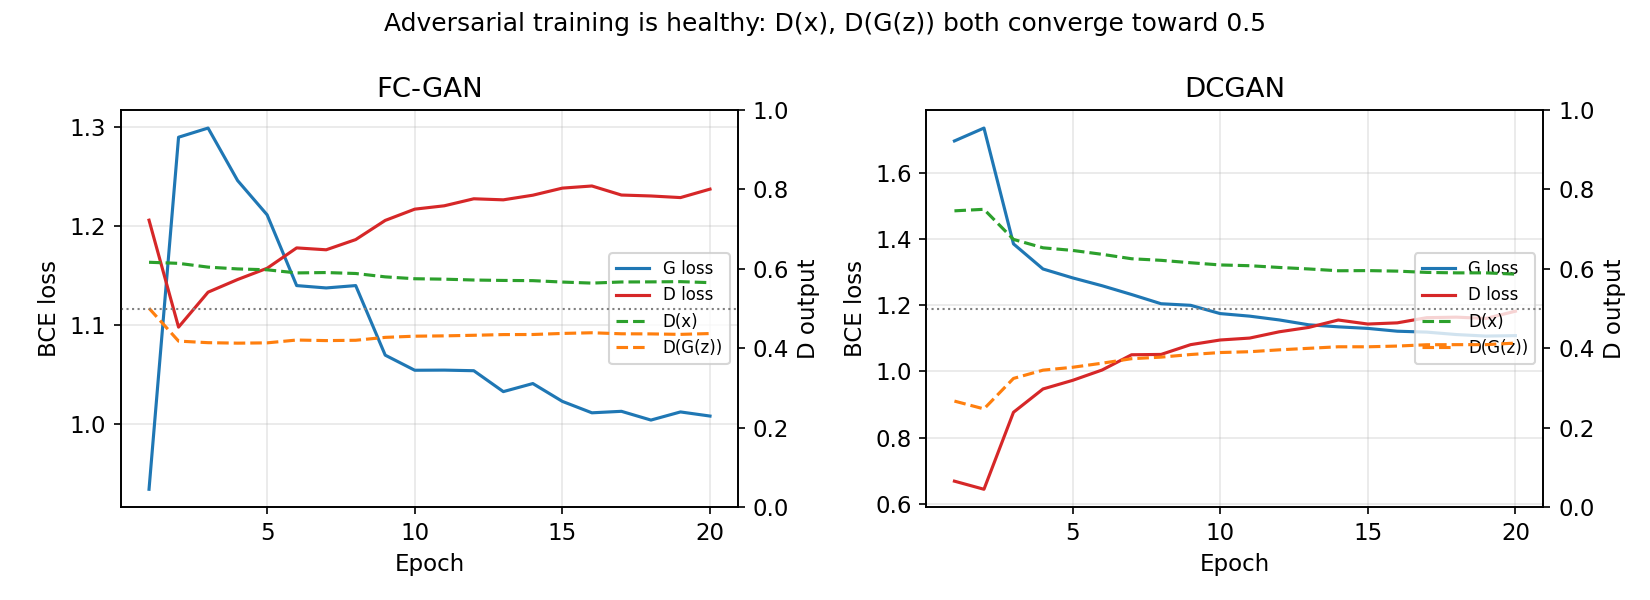
\includegraphics[width=\textwidth]{gan_losses.png}
  \caption{FC-GAN（左）与 DCGAN（右）的训练损失（实线）与判别器输出 $D(x)$、$D(G(z))$（虚线，向 0.5 收敛），表明对抗训练健康。}
  \label{fig:losses}
\end{figure}


\subsection{DCGAN 与 CelebA 扩展}
DCGAN 以相同设置训练 20 个 epoch（损失见图~\ref{fig:losses} 右），一组随机噪声下生成质量明显高于全连接版本，定量与可视化对比见第~\ref{sec:cmp}~节。为检验框架可扩展性，我们另在 \textbf{CelebA}（202{,}599 张人脸，$64\times64$ RGB）上训练 5 个 epoch 的加深版 DCGAN（5 层卷积/转置卷积），生成的人脸已能呈现大致的五官布局与肤色光影（图~\ref{fig:celeba}；5 epoch 仍偏粗糙、局部有扭曲），说明同一套对抗训练框架可迁移到更高分辨率的彩色图像。

\begin{figure}[H]
  \centering
  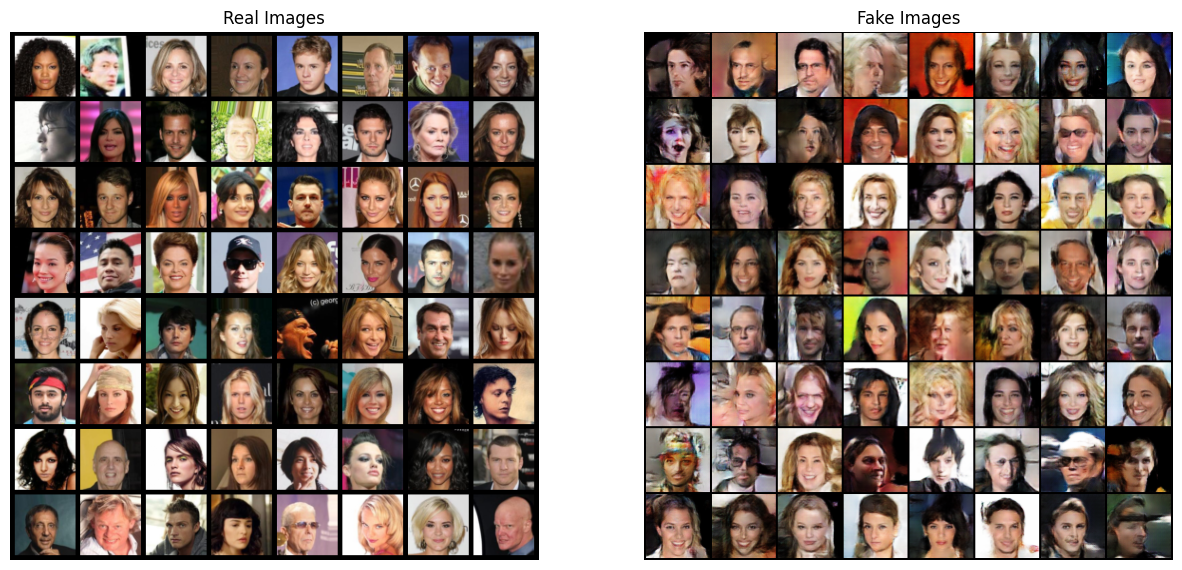
\includegraphics[width=0.62\textwidth]{celeba_real_fake.png}
  \caption{CelebA 上 DCGAN 的真实人脸（左）与生成人脸（右），5 epoch。}
  \label{fig:celeba}
\end{figure}

\section{分析与讨论}
\label{sec:cmp}
表~\ref{tab:cmp} 汇总全连接 GAN 与 DCGAN 的最终指标，图~\ref{fig:cmp} 用同一组 16 个噪声直观对比二者的生成质量。

\begin{table}[H]
  \centering
  \caption{全连接 GAN 与 DCGAN 对比（第 20 epoch 的 epoch 均值）}
  \label{tab:cmp}
  \begin{tabular}{lrrrrr}
    \toprule
    模型 & $G$ 参数量 & $D$ 参数量 & $G$ loss & $D$ loss & $D(x)\,/\,D(G(z))$ \\
    \midrule
    全连接 GAN & 560{,}656 & 233{,}985 & 1.008 & 1.237 & 0.566 / 0.437 \\
    DCGAN（卷积） & 1{,}781{,}504 & 138{,}624 & 1.108 & 1.181 & 0.587 / 0.413 \\
    \bottomrule
  \end{tabular}
\end{table}

\begin{figure}[H]
  \centering
  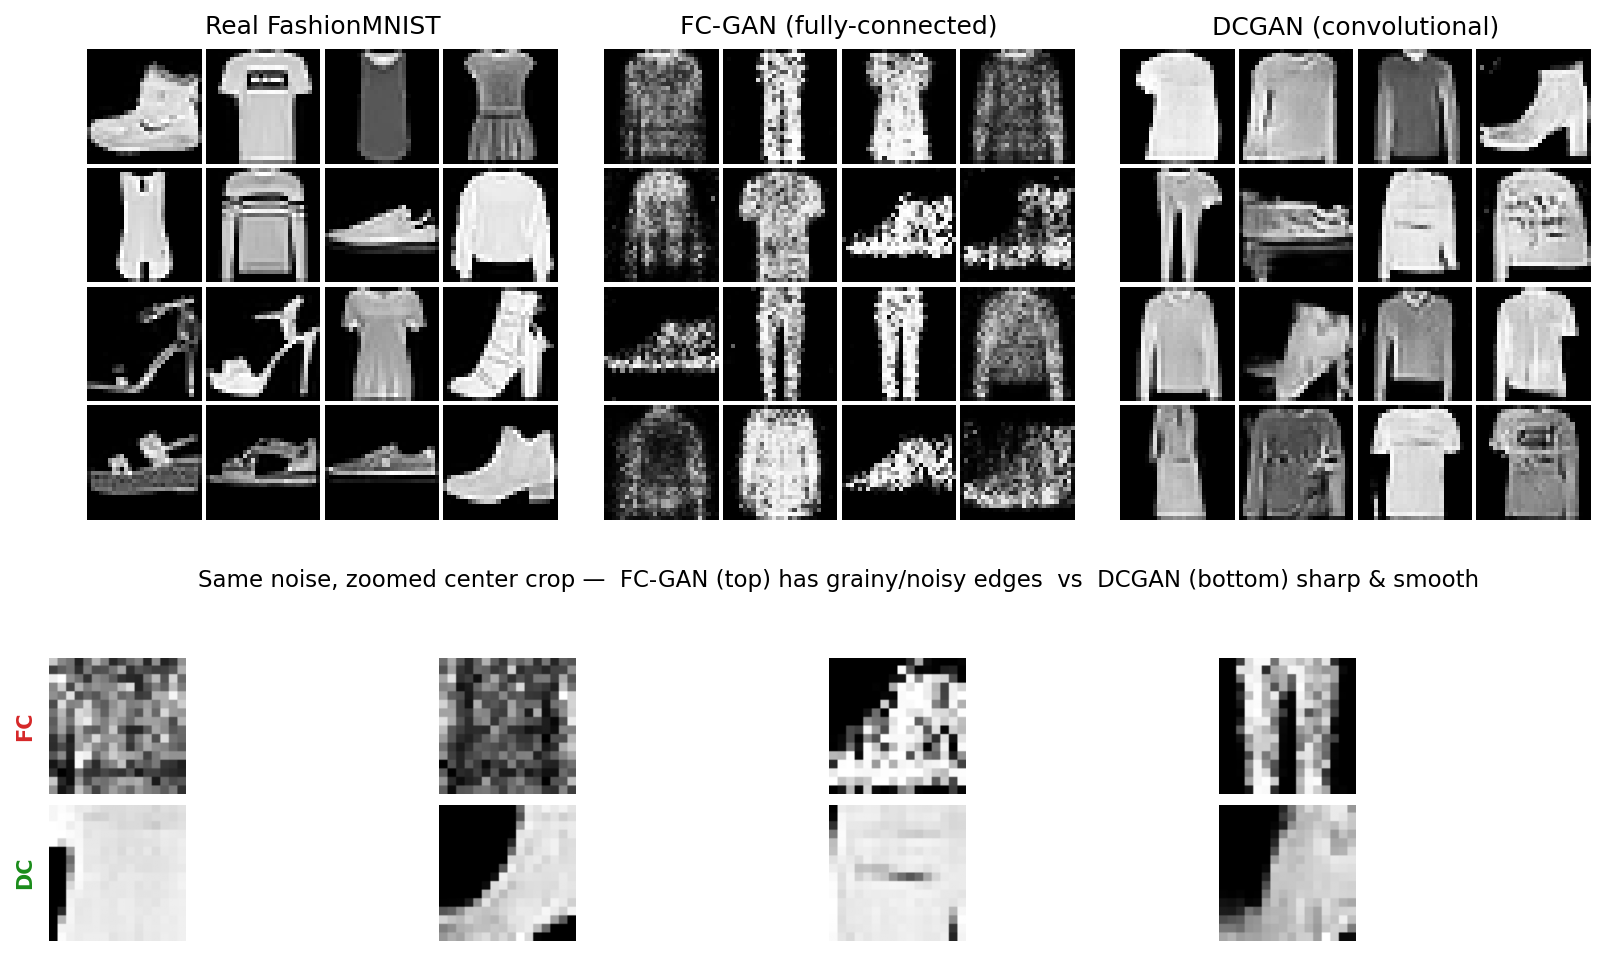
\includegraphics[width=0.9\textwidth]{exp4_quality.png}
  \caption{生成质量对比。上：真实图 / FC-GAN / DCGAN（FC 与 DC 用同一组 16 个噪声）；下：同一噪声的中心局部放大——FC-GAN 边缘颗粒噪点明显，DCGAN 锐利平滑。}
  \label{fig:cmp}
\end{figure}

两者的损失数值相近——这是对抗损失的特点，它衡量的是博弈状态而非绝对生成质量——但\textbf{视觉质量差距显著}：DCGAN 生成的衣物边缘锐利、明暗过渡自然、几乎没有椒盐噪点，裤腿、鞋型、衣领等局部结构清晰；FC-GAN 则普遍带有颗粒噪声、轮廓发虚。原因在于卷积结构的\textbf{空间归纳偏置}：转置卷积的局部感受野与权重共享让相邻像素天然相关，生成图像局部平滑、结构连贯；而全连接层把 784 个像素当作彼此独立的输出维度，必须靠数据"硬学"像素间的空间相关性，因此更容易出现噪点。

\textbf{从生成器内部看卷积的作用.} 进一步可视化 DCGAN 生成器的中间特征图（图~\ref{fig:featmaps}）：噪声 $\bm{z}$ 先被转置卷积投影成 $256$ 个 $7\times7$ 的\textbf{粗特征}（勾勒大致轮廓与布局），再经两层 stride-2 转置卷积上采样为 $128$ 个 $14\times14$ 的\textbf{中层特征}（细化边缘与局部结构），最后合成 $28\times28$ 的图像。这种“由粗到细、逐级上采样”的合成过程正是卷积生成器优于全连接的本质：空间结构是\textbf{逐层、局部地}被构造出来的，而非由全连接层一次性把每个像素独立预测出来。

\begin{figure}[H]
  \centering
  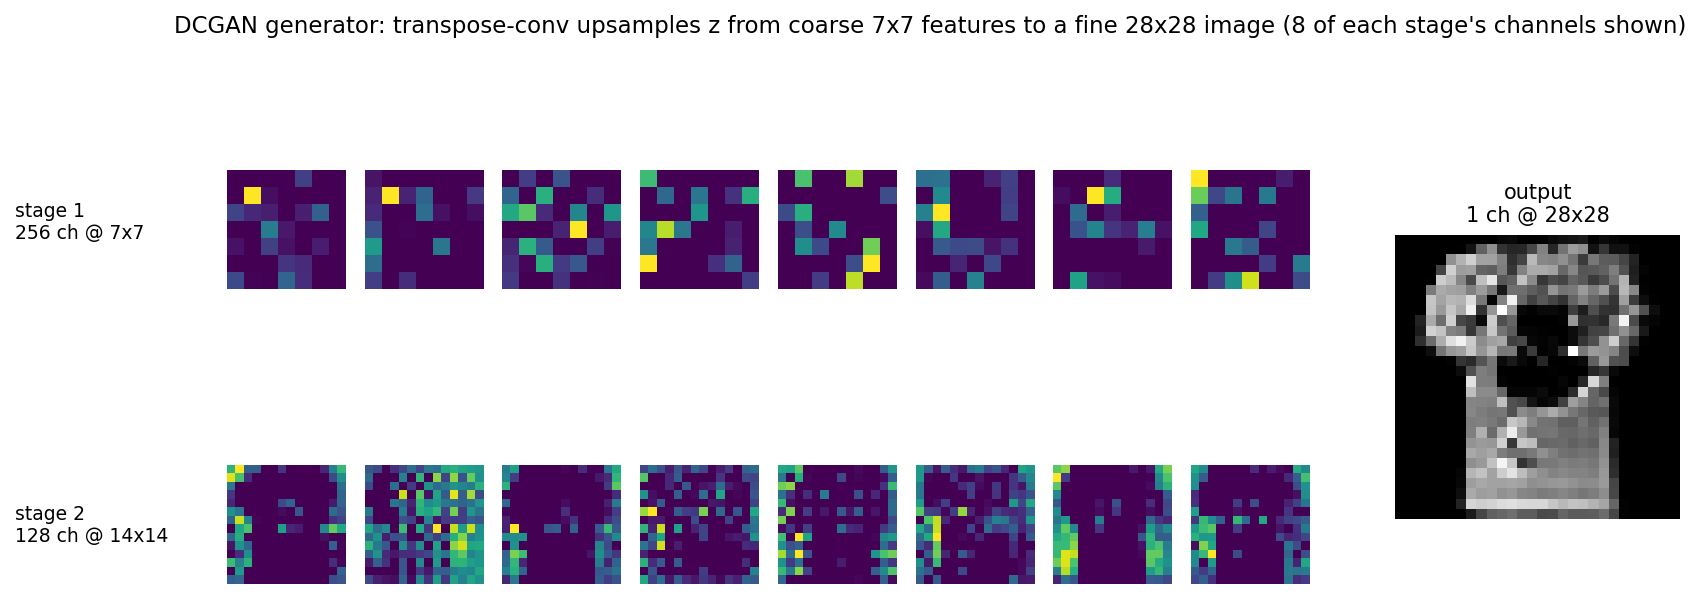
\includegraphics[width=\textwidth]{exp4_featmaps.png}
  \caption{DCGAN 生成器中间特征图：$\bm{z}\to 7\times7$（256 通道，粗轮廓）$\to 14\times14$（128 通道，细化）$\to 28\times28$ 输出（各阶段展示 8 个通道）。}
  \label{fig:featmaps}
\end{figure}

\subsection{随机数调整对生成结果的影响}

固定随机种子 123 采样 8 个 100 维标准正态噪声，生成结果见图~\ref{fig:trav}(a)：可辨认出包、裤子、套衫、鞋等类别，整体轮廓正确但边缘有颗粒噪点（全连接缺乏空间归纳偏置的典型表现）。以这 8 个噪声为基准（对应 8 列），从 100 维中挑选第 $\{5,25,45,65,85\}$ 共 5 个维度、每维取 $\{-2.5,0,+2.5\}$ 三档（其余 99 维不变），得到图~\ref{fig:trav}(b) 的 $15\times8$ 扰动网格（每 3 行一组对应一个维度）。逐维观察可归纳出三点现象（成因见下文）：单维扰动引起整张图的\textbf{整体渐变}而非孤立属性变化；基准噪声决定类别、单维扰动多在类内形变，仅在 $\pm2.5$ 时偶尔把样本推过类别边界（鞋$\leftrightarrow$靴过渡）；幅度越大变化越剧烈、噪点越多，不同维度作用方向也各不相同。

\begin{figure}[H]
  \centering
  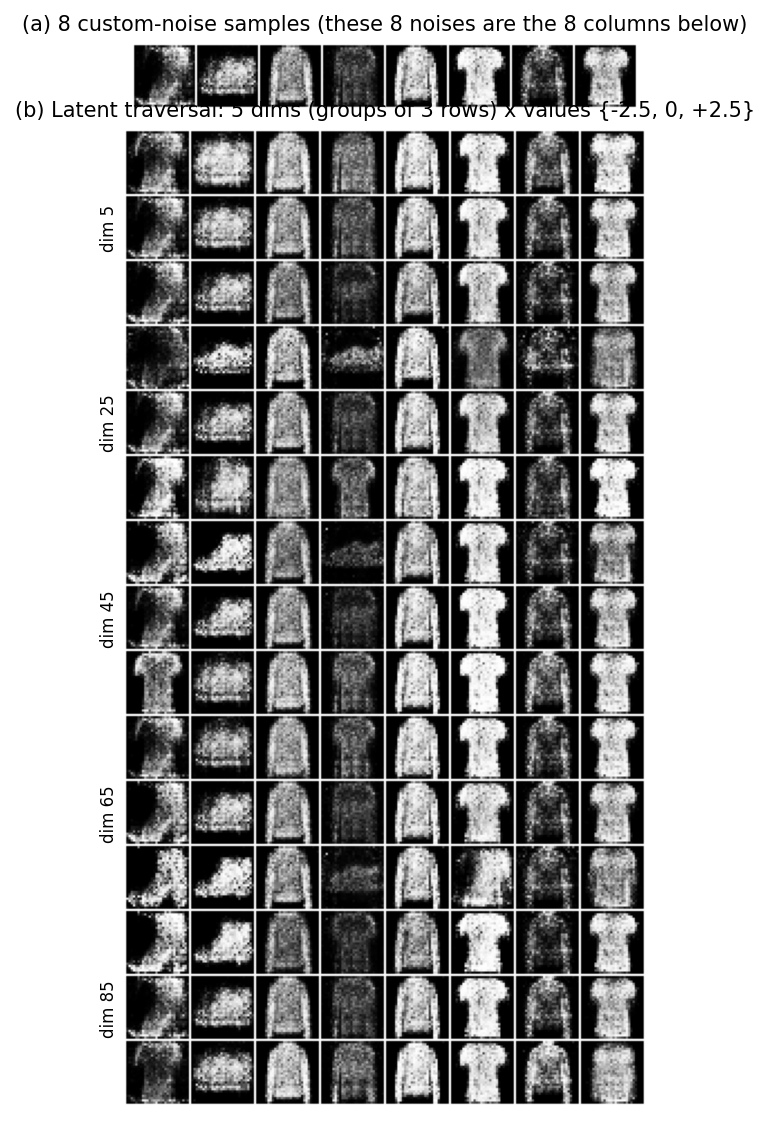
\includegraphics[width=0.56\textwidth]{fc_traversal_full.png}
  \caption{(a) 8 个自定义噪声样本；(b) 以同样 8 个噪声为列的 $15\times8$ 潜变量扰动（每 3 行一组对应一个维度，组内取值 $-2.5/0/+2.5$）。}
  \label{fig:trav}
\end{figure}

结合 $15\times8$ 扰动实验，对"调整随机数如何影响生成结果"总结如下：
\begin{itemize}
  \item \textbf{噪声 $\bm{z}$ 是生成图像唯一的信息来源，其整体位置决定生成什么}。生成器学到的是从 100 维标准正态分布到图像流形的连续映射 $G:\mathbb{R}^{100}\rightarrow\mathbb{R}^{28\times28}$。8 个基准噪声落在流形的不同区域，因此分别对应包、裤子、套衫、鞋等不同类别——"类别"这一最主要的语义由 $\bm{z}$ 的整体位置决定，而非某一维单独决定。
  \item \textbf{普通 GAN 的潜空间是纠缠的：单个维度不对应单个语义属性}。实验中调整任何一维，都观察到亮度、形状、纹理的\textbf{联动渐变}，找不到一个只控制袖长或只控制明暗的维度。这是因为标准 GAN 的训练目标只要求生成分布逼近数据分布，对潜空间的组织方式没有任何约束，各语义因子自然地以混合的方式分布在所有维度上（这正是 InfoGAN、StyleGAN 等后续工作引入解耦约束的动机）。
  \item \textbf{$G$ 是连续映射，因此扰动带来的是平滑过渡}。取值从 $-2.5$ 经 0 到 $+2.5$，图像呈连续形变而非跳变；只有当扰动把 $\bm{z}$ 推过两个类别在潜空间中的边界时，才会看到鞋$\leftrightarrow$靴这类离散的类别切换，且切换附近往往出现"两类之间"的模糊形态。
  \item \textbf{扰动幅度与生成质量的关系印证了训练分布的作用}。$|z_d|\leq 1$ 附近（标准正态的高密度区）生成质量最好；取到 $\pm2.5$ 时图像变化剧烈且噪点增多，因为训练时几乎采不到这些低密度区域的样本，生成器在那里的映射没有得到充分学习。
  \item \textbf{同一维度对不同基准噪声的影响不同}。这说明 $G$ 学到的映射是高度非线性的：某一维的"语义方向"依赖于 $\bm{z}$ 所处的局部邻域，在流形的不同区域，同一坐标轴方向对应不同的图像变化。
\end{itemize}

\textbf{潜空间插值与截断：另外两种“调随机数”的视角.} 除单维扰动外，我们再用两种方式考察噪声的影响（图~\ref{fig:noise}，用 DCGAN 生成）。\textbf{球面插值}：在两个随机噪声之间做球面线性插值，生成结果\textbf{平滑地从一种衣物过渡到另一种}、没有突兀跳变——直观证明 $G$ 是从噪声到图像的连续映射。\textbf{截断技巧}：把噪声整体乘以系数 $\sigma$，$\sigma$ 越小（采样越集中于分布中心）生成越规整但越雷同（保真度高、多样性低），$\sigma$ 越大越多样但畸变与噪点增多——这与上面“高密度区质量好、低密度区质量差”的结论互相印证，也是 BigGAN 等工作中“截断换保真”技巧的由来。

\begin{figure}[H]
  \centering
  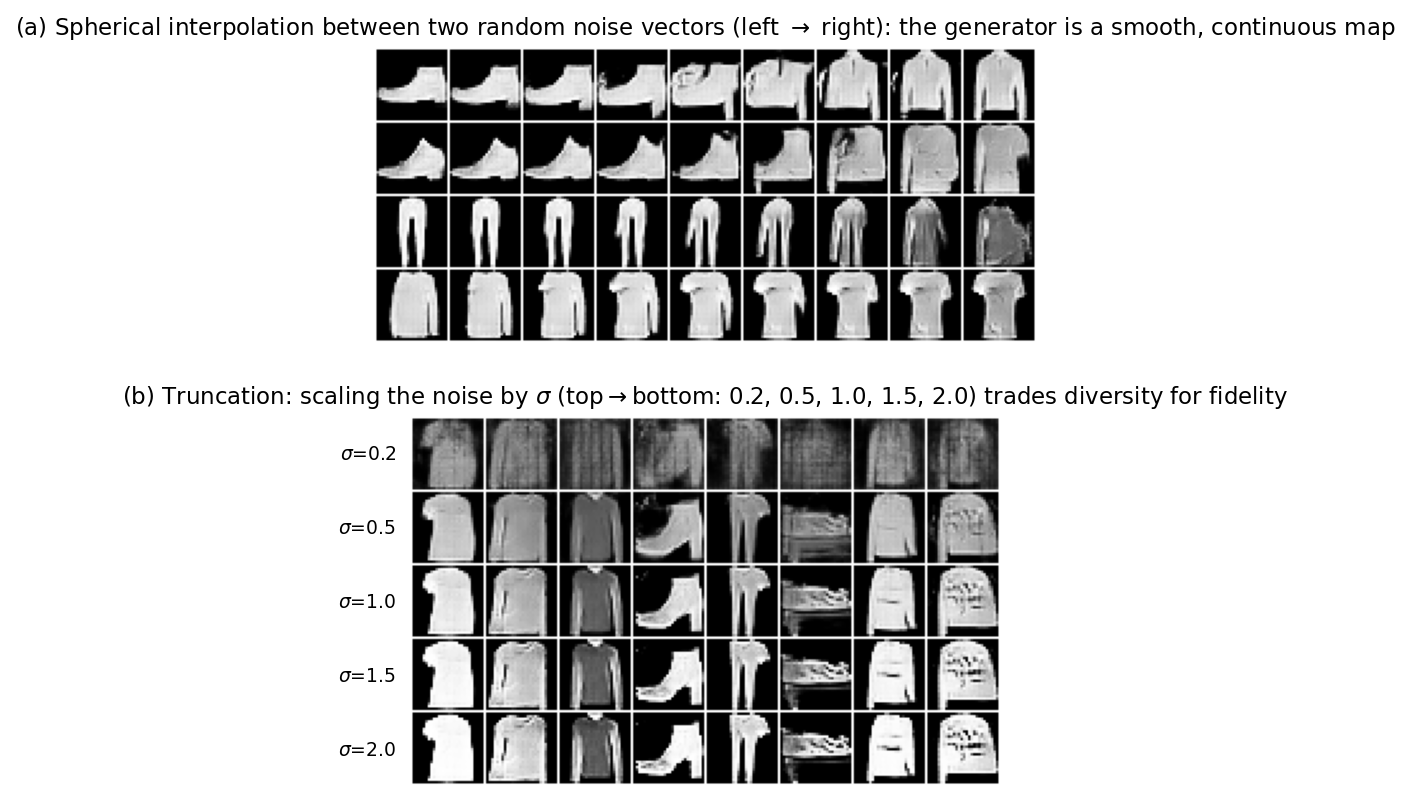
\includegraphics[width=\textwidth]{exp4_noise.png}
  \caption{随机数影响的另外两种视角（DCGAN）。(a) 两个噪声间的球面插值：生成图像连续过渡，说明 $G$ 是连续映射；(b) 噪声幅度 $\sigma$ 由小到大：保真度与多样性此消彼长。}
  \label{fig:noise}
\end{figure}

此外，本实验对 GAN 的训练动态也有直观体会：判别器输出 $D(x)$、$D(G(z))$ 最终都在 0.5 两侧（DCGAN 尤其呈清晰的双向收敛）、损失曲线呈拉锯而非单调下降，是对抗训练健康进行的标志；而 DCGAN 与 FC-GAN 损失数值接近、视觉质量却差距明显，提醒我们\textbf{对抗损失不能直接当作生成质量的度量}，结构先验（卷积）对生成图像质量起着决定性作用。

\subsection{GAN 的模式崩溃问题}
\label{sec:collapse}
在GAN对抗生成时常会遇到模式崩溃问题，模式崩溃（mode collapse）指生成器只学会产出少数几种样本、覆盖不了真实数据的全部模态。其根源在于 GAN 的极小极大博弈：生成器的目标只是“骗过\textbf{当前}判别器”，一旦它找到某几个能稳定骗过 $D$ 的输出，就会把大量不同的噪声 $\bm{z}$ 都映射到这几个输出上，从而丢失多样性；当 $D$ 与 $G$ 的更新失衡（如 $D$ 过弱、学习率不当）或缺乏稳定化手段时尤其容易发生。

为直观展示，我们在相同数据上训练两个全连接 GAN：一个采用\textbf{健康设置}（生成器带 BatchNorm、$G/D$ 学习率平衡、$1{:}1$ 更新），另一个去掉生成器 BatchNorm、判别器学习率调低且每步多更新生成器故意制造失衡。训练后各采样 2000 张，用一个在 FashionMNIST 上训练的小型 CNN 分类器统计生成样本落入 10 个类别的分布（图~\ref{fig:collapse}）。结果非常清晰：健康模型的生成样本\textbf{覆盖全部 10 类}（类别分布熵 $2.16$，接近均匀上限 $\ln 10\approx2.30$）；崩溃模型则\textbf{几乎只生成 Sandal 与 Shirt 两类}（熵骤降到 $0.68$），其余 8 类几乎从不出现——这正是模式崩溃的典型表现，且生成质量也随之劣化。

\begin{figure}[H]
  \centering
  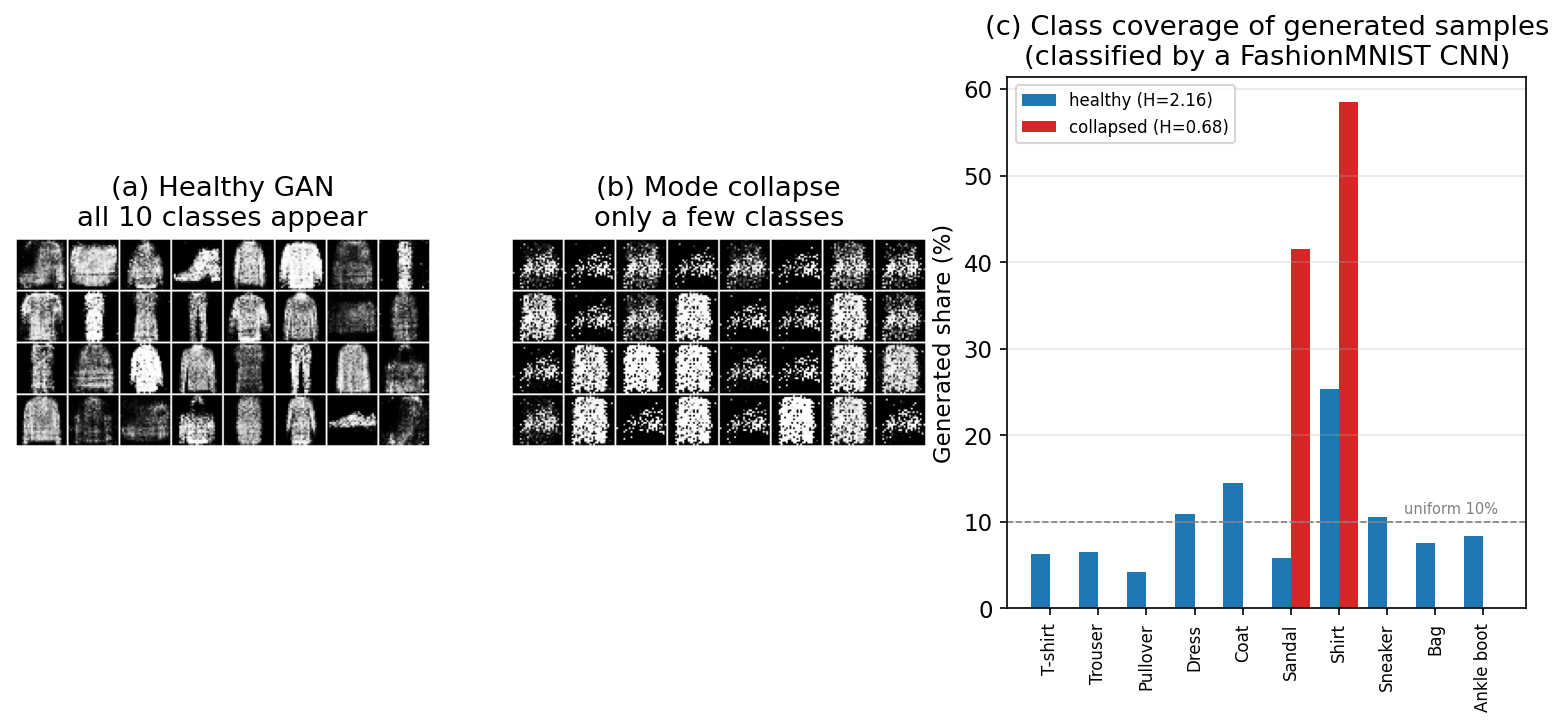
\includegraphics[width=\textwidth]{mc_collapse.png}
  \caption{模式崩溃演示。(a) 健康 GAN 样本；(b) 崩溃 GAN 样本；(c) 用 FashionMNIST 分类器统计的生成类别分布——健康模型覆盖 10 类（熵 $2.16$），崩溃模型几乎只产出 2 类（熵 $0.68$）。}
  \label{fig:collapse}
\end{figure}

缓解模式崩溃的主要思路包括：(1) \textbf{改进损失/距离度量}，如 WGAN、WGAN-GP 以 Wasserstein 距离提供更平滑、不易饱和的梯度；(2) \textbf{让判别器“看到”批内多样性}，如 minibatch discrimination、feature matching，使 $D$ 能惩罚“整批雷同”；(3) \textbf{稳定化训练技巧}，如谱归一化（spectral norm）、双时间尺度更新（TTUR）、单边标签平滑、给 $D$ 输入加噪；(4) \textbf{结构与更新平衡}，保持 $G/D$ 容量与更新频率匹配、生成器使用 BatchNorm。

\section{结论}
本次实验我们在 FashionMNIST 上实现并对比了全连接 GAN 与卷积 DCGAN，并围绕随机数对生成的影响和模式崩溃两个重点展开探究与讨论。主要结论有三：其一，两套模型的 $D(x)$、$D(G(z))$ 最终都落在 0.5 两侧（DCGAN 双向收敛尤为明显），对抗博弈健康，但损失数值相近、视觉质量却差距明显，说明\textbf{对抗损失不能直接当作生成质量的度量}，卷积的空间归纳偏置更可能是 DCGAN 质量更优的原因。其二，噪声 $\bm{z}$ 是生成的唯一信息来源：其整体位置决定生成类别，单维扰动引起整体的平滑渐变而非独立属性变化，普通 GAN 的潜空间高度\textbf{纠缠}，插值与截断实验进一步印证了 $G$ 是连续映射、且高密度区生成质量更好。其三，通过失衡训练复现了\textbf{模式崩溃}，并讨论了 WGAN-GP、minibatch discrimination、谱归一化等对策。

\begin{thebibliography}{9}
  \bibitem{gan} I.~Goodfellow, J.~Pouget-Abadie, M.~Mirza, et al. Generative Adversarial Nets. \textit{NeurIPS}, 2014.
  \bibitem{dcgan} A.~Radford, L.~Metz, S.~Chintala. Unsupervised Representation Learning with Deep Convolutional Generative Adversarial Networks. \textit{ICLR}, 2016.
  \bibitem{fashionmnist} H.~Xiao, K.~Rasul, R.~Vollgraf. Fashion-MNIST: a Novel Image Dataset for Benchmarking Machine Learning Algorithms. \textit{arXiv:1708.07747}, 2017.
  \bibitem{tutorial} N.~Inkawhich. DCGAN Tutorial. PyTorch Tutorials.
\end{thebibliography}

\end{document}